\documentclass[border=8pt]{standalone}
\usepackage[utf8]{inputenc}
\usepackage{tikz}
\usetikzlibrary{positioning}

\tikzset{
  entita/.style = {rectangle, draw, thick, fill=blue!8, minimum width=30mm, minimum height=16mm, font=\small},
  attr/.style   = {circle, draw, thick, fill=white, minimum size=5pt, inner sep=0},
  pk/.style     = {circle, draw, thick, fill=black, minimum size=5pt, inner sep=0},
  link/.style   = {thick},
  et/.style     = {font=\footnotesize}
}

\begin{document}
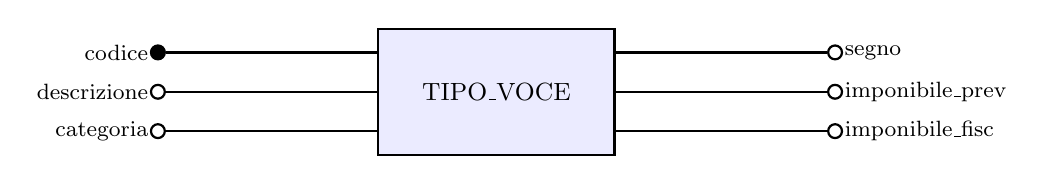
\begin{tikzpicture}
  \node[entita] (E) {TIPO\_VOCE};

  \node[pk]   (c)  at (-4.3, 0.5){}; \draw[link] (-1.5, 0.5)--(c);  \node[et,left] at (c)  {codice};
  \node[attr] (d)  at (-4.3, 0.0){}; \draw[link] (-1.5, 0.0)--(d);  \node[et,left] at (d)  {descrizione};
  \node[attr] (ca) at (-4.3,-0.5){}; \draw[link] (-1.5,-0.5)--(ca); \node[et,left] at (ca) {categoria};

  \node[attr] (s)  at (4.3, 0.5){}; \draw[link] (1.5, 0.5)--(s);  \node[et,right] at (s)  {segno};
  \node[attr] (ip) at (4.3, 0.0){}; \draw[link] (1.5, 0.0)--(ip); \node[et,right] at (ip) {imponibile\_prev};
  \node[attr] (if) at (4.3,-0.5){}; \draw[link] (1.5,-0.5)--(if); \node[et,right] at (if) {imponibile\_fisc};
\end{tikzpicture}
\end{document}
